% main.tex -- PNAS Research Article
% Training-Free Generation of Protein Sequences via Stochastic Attention
% NOTE: PNAS accepts format-neutral initial submissions.
% Single-column with line numbers for reviewer readability.
% Switch to twocolumn + pnasresearcharticle for final production.
\pdfminorversion=7
\documentclass[11pt,onecolumn,twoside,lineno]{pnas-new}
\templatetype{pnasresearcharticle}

\usepackage{amsmath,amssymb}
\usepackage{multirow}
\usepackage{algorithm}
\usepackage[noend]{algpseudocode}

% Metadata
\title{Training-Free Generation of Protein Sequences from Small Family Alignments via Stochastic Attention}

\author[a,1]{Jeffrey D. Varner}
\affil[a]{R.F. Smith School of Chemical and Biomolecular Engineering, Cornell University, Ithaca, NY 14850}

\leadauthor{Varner}

\significancestatement{Most protein families have fewer than 100 known members, too few to train a deep generative model. We show that a single attention operation over a family alignment defines an energy landscape whose Boltzmann distribution can be sampled via Langevin dynamics, with no training, no GPU, and no external data. The resulting method, stochastic attention, generates novel protein sequences that preserve family-level amino acid statistics and are predicted by independent structure predictors to adopt the correct fold across eight diverse families. A simple linear relationship between representation dimensionality and the critical sampling temperature enables fully automatic operation from a seed alignment, opening training-free sequence generation to the majority of protein families too small for deep learning.}

\authorcontributions{J.D.V.\ designed research, performed research, analyzed data, and wrote the paper.}
\authordeclaration{The author declares no competing interest.}
\correspondingauthor{\textsuperscript{1}To whom correspondence should be addressed. E-mail: jdv27@cornell.edu. ORCID: 0000-0002-2558-7026.}

\keywords{protein sequence generation $|$ stochastic attention $|$ Hopfield networks $|$ Langevin dynamics $|$ training-free generative models}

\dates{This manuscript was compiled on \today}
\doi{\url{https://doi.org/10.1073/pnas.XXXXXXXXXX}}

\begin{document}

\begin{abstract}
Generating novel protein sequences that respect the statistical constraints of a family typically requires training deep generative models on thousands to millions of examples. Yet most protein families are small: the median Pfam family has fewer than 100 members, a regime where learned models overfit or collapse. We propose \emph{stochastic attention} (SA), a training-free sampler that treats the modern Hopfield energy over stored protein sequences as a Boltzmann distribution and draws samples via Langevin dynamics. The score function is given in closed form by the residual of a single softmax attention operation, eliminating the need for a trained score network, external pretraining data, or graphics processing unit (GPU) resources. Across eight Pfam families spanning 37 to 420 sequences and 23 to 262 residues, SA generates sequences with low amino acid composition divergence, substantial novelty, and structural plausibility confirmed by ESMFold and AlphaFold2. Head-to-head comparison with profile HMMs, EvoDiff, and the MSA Transformer shows that SA is the only method to simultaneously achieve low composition divergence, genuine novelty, and sequence identity within the natural within-family range ($30$--$70\%$); competing methods either drift outside the family or produce near-copies of stored patterns. The critical inverse temperature is predicted from principal component analysis (PCA) dimensionality alone with high accuracy, enabling fully automatic operation from a seed alignment. Independent validation by ESM2-650M and cross-referencing against deep mutational scanning experiments confirm that over 90 percent of SA-generated substitutions correspond to experimentally tolerated mutations.
\end{abstract}

\maketitle
\thispagestyle{firststyle}

\dropcap{W}ith protein structure prediction largely solved by AlphaFold2~\cite{jumperHighlyAccurateProtein2021} and RoseTTAFold~\cite{baekRoseTTAFold2021}, the frontier has shifted toward \emph{designing} novel protein sequences with desired properties~\cite{kuhlmanBradleyAdvances2019,huangComingAgeDeNovo2016}. Generative approaches now span a broad landscape, from classical profile hidden Markov models (pHMMs)~\cite{hmmer3,kroghHiddenMarkovModels1994} and Potts models~\cite{morcosDirectCouplingAnalysis2011,ekeberg2013improved,trinquierEfficientGenerativeModeling2021} to deep generative models including variational autoencoders~\cite{kingmaWellingAutoEncoding2014,riesselman2018deep}, autoregressive language models~\cite{ferruzProtGPT2DeepUnsupervised2022,madaniProGenLanguageModeling2023}, alignment-processing transformers~\cite{raoMSATransformer2021}, MSA-conditioned diffusion~\cite{alamdariProteinGeneration2023}, and structure-conditioned methods such as ProteinMPNN~\cite{dauparasProteinMPNN2022} and RFdiffusion~\cite{watsonRFdiffusion2023}. Yet all sequence-level approaches share a common requirement: large training corpora. Language models are pretrained on millions of UniRef50 sequences; even MSA-conditioned methods require either extensive pretraining or large input alignments. This reliance on scale creates a fundamental blind spot, because the median Pfam family contains fewer than 100 full-length members~\cite{mistryPfamProteinFamilies2021} and thousands of families have fewer than 50. In this scarce-data regime, deep models overfit and collapse in diversity, while pHMMs emit sequences that drift far from the family's functional envelope. What is needed is an approach that can extract the statistical structure of a protein family from whatever data is available, even a few dozen sequences, without learning parameters that could overfit.

A separate line of work provides exactly this capability. Ramsauer et al.~\cite{ramsauerHopfieldNetworksAll2021} showed that a single softmax attention operation is equivalent to one step of the retrieval dynamics on the modern Hopfield energy, building on the dense associative memory framework of Krotov and Hopfield~\cite{krotovDenseAssociativeMemory2016}. This connection endows any set of stored examples with a well-defined energy landscape: the examples become memory patterns, and the Boltzmann distribution over this landscape assigns high probability to states that resemble the stored set. Critically, the Hopfield energy provides the score function \emph{analytically}, as the residual of a single attention operation, so Langevin sampling can proceed without learning any parameters. We exploit this insight to propose \emph{stochastic attention} (SA), a training-free protein sequence generator that combines the exact Hopfield score function with Langevin dynamics. Our prior work~\cite{alswaidanVarnerStochasticAttention2026} introduced SA and validated it on synthetic data, MNIST, and a single protein family.

In this study, we explored the extent to which stochastic attention can serve as a practical generative model for real protein families. We systematically evaluated SA across eight diverse Pfam families spanning a ten-fold range of family sizes and a seven-fold range of sequence lengths, assessing compositional fidelity, sequence novelty, and structural plausibility using both ESMFold and AlphaFold2. We characterized how generation quality scales with family size, uncovering an empirical law that predicts the critical temperature from alignment statistics alone and eliminates the need for a temperature sweep. We tested robustness in the extreme scarce-data regime down to $K{=}20$ sequences, compared SA head-to-head against four established baselines (profile HMMs, EvoDiff, MSA Transformer, and a Potts model), and examined whether the generated sequences preserve the pairwise residue covariation that reflects structural contacts and functional couplings. Finally, we sought independent validation of biological plausibility through ESM2-650M pseudo-perplexity scoring and cross-referencing against published deep mutational scanning datasets.

\section*{Results}

We ran stochastic attention on all eight Pfam families (Table~\ref{tab:families}) and observed that the method consistently generated novel protein sequences while preserving family-level amino acid statistics, across a ten-fold range of family sizes and a seven-fold range of sequence lengths (Fig.~\ref{fig:cross-family}; SI Appendix, Table~S1). We first confirmed that the sampler converged to the correct Boltzmann distribution by comparing the outputs of the unadjusted Langevin algorithm (ULA) and its Metropolis-adjusted variant (MALA): acceptance rates exceeded 99.6\% in every family (SI Appendix, Table~S7), confirming negligible discretization bias and justifying the use of the computationally cheaper ULA in all subsequent experiments. Generated sequences were not near-duplicates of stored patterns: zero sequences across all eight families exceeded 90\% identity to any stored sequence (SI Appendix, Table~S9), and the generated ensemble was insensitive to initialization strategy (SI Appendix, Table~S8). In the generation regime (inverse temperature $\beta \approx 2\beta^*$, just above the entropy inflection point where pattern-specific basins first emerge), SA achieved Kullback--Leibler (KL) divergences below $0.06$ in every family, with several below $0.02$. Novelty ranged from $0.40$ (Defensin\_beta) to $0.65$ (WW), indicating substantial departure from any single stored memory, and mean pairwise cosine distance was ${\approx}1.0$ in every family, confirming that the sampler produced distinct, well-separated sequences rather than collapsing to a single mode. Nearest sequence identity to a stored pattern was $51$--$66\%$, comparable to the typical within-family identity range, indicating that generated sequences remained within the family's functional envelope while departing meaningfully from stored patterns. By contrast, bootstrap samples had zero novelty by construction and Gaussian perturbation produced negligible novelty ($<0.02$), confirming that small additive noise is insufficient to escape the basin of the nearest stored pattern.

To understand why SA preserves these statistics, we examined the position-specific behavior of the sampler in the Kunitz domain (SI Appendix, Fig.~S5). SA-generated sequences preserved all 11 positions with greater than 90\% conservation in the seed alignment, including all six cysteines forming the three disulfide bonds essential to the Kunitz fold, while introducing 17--25 substitutions concentrated at variable positions. Per-position Shannon entropy correlated strongly between the SA-generated ensemble and the stored alignment ($r{=}0.968$), confirming that the method correctly identifies which positions tolerate variation and which do not. This behavior is a direct consequence of the Boltzmann sampling mechanism: at strongly conserved positions, all stored patterns agree and the softmax weights concentrate probability on the consensus residue; at variable positions, stored patterns diverge and the sampler draws from the local distribution of tolerated amino acids.

To characterize how generation quality degrades with decreasing family size, we subsampled the WW domain at $K \in \{20, 50, 100, 200, 400\}$ with five independent replicates per condition (SI Appendix, Fig.~S2). Stochastic attention maintained low KL divergence across the entire range ($0.019 \pm 0.008$ at $K{=}20$, improving to $0.010 \pm 0.002$ at $K{=}400$), while the PCA dimensionality grew from $d{=}17$--$18$ components at $K{=}20$ to $d{=}182$--$183$ at $K{=}400$ and the critical temperature tracked this growth ($\beta^*{=}2.7$ to $5.5$). Despite the roughly ten-fold increase in effective dimensionality, SA generation quality remained stable, suggesting that the entropy inflection criterion successfully adapted the operating temperature to the geometry of the memory matrix at each scale. Novelty increased with $K$ (from $0.47$ to $0.74$), reflecting the richer landscape of a larger memory set, while nearest sequence identity decreased correspondingly (from $0.71$ to $0.56$), indicating that the sampler explored further from stored patterns when more patterns were available to collectively shape the energy landscape. Replication across three additional families at $K{=}20$ (SH3, Kunitz, zf-C2H2) confirmed that this robustness is not family-specific (SI Appendix, Table~S2).

The scaling study revealed that $\beta^*$ tracks PCA dimensionality; we next asked whether this relationship could be predicted from alignment statistics alone, without running an explicit temperature sweep (Fig.~\ref{fig:beta-prediction}). We pooled 33 data points (the 8 Pfam families and 25 WW scaling replicates) and found that a simple two-parameter model, $\beta^* \approx 1.57 + 0.28\sqrt{d}$ (bootstrap standard error [SE]: intercept $\pm 0.07$, slope $\pm 0.007$), explained 97\% of the variance ($R^2{=}0.97$). The intercept of $1.57$ recovers the universal softmax inflection baseline, and the fitted slope of $0.28$ is roughly half the $\sqrt{d}$ coefficient predicted for random patterns. This reduction arises from two effects: concentration of measure on $\mathbb{S}^{d-1}$ guarantees that cross-similarities between stored patterns scale as $\mathcal{O}(1/\sqrt{d})$, setting the $\sqrt{d}$ dependence, while self-similarity anchoring (each stored pattern has unit inner product with itself, creating a gap of $0.55$--$0.82$ over the next-nearest pattern) shifts the inflection to lower $\beta$ than a Gaussian mean-field model predicts; together these effects reflect the structured similarity spectrum of real protein sequences arising from conserved positions, correlated substitutions, and phylogenetic signal (SI Appendix, Section~S18). Adding further predictors (mean column entropy, effective number of sequences, spectral concentration) produced negligible improvement ($\Delta R^2 < 0.001$), indicating that PCA dimensionality captures most of the relevant variation. Refitting on the eight Pfam families alone yielded a nearly identical relationship ($R^2{=}0.95$), confirming that the result is not driven by overrepresentation of the WW family. This regression provides a practical shortcut: given a new family, one can estimate $\beta^*$ from PCA alone and set the generation temperature without a sweep.

We compared stochastic attention against three established learned baselines, profile HMM emit, EvoDiff (MSA-conditioned diffusion), and the MSA Transformer (Gibbs masked language model sampling), across all eight families (Fig.~\ref{fig:baseline-comparison}). Reading the three panels jointly is essential: no single metric tells the full story, and a method that scores well on novelty while failing on compositional fidelity or sequence identity has simply generated sequences that no longer belong to the family. Profile HMM emit and the MSA Transformer achieved high novelty scores, but this apparent advantage is illusory: their nearest sequence identity to stored patterns fell to $11$--$59\%$ in several families, well below the typical within-family range of $30$--$70\%$ (shaded band, Fig.~\ref{fig:baseline-comparison}C). Sequences below this range have drifted outside the family and are unlikely to retain its function; sequences above it are near-copies of stored patterns with insufficient novelty. The high novelty of HMM emit and the MSA Transformer reflects compositional drift, not meaningful exploration of family sequence space. EvoDiff balanced the metrics more effectively in shorter families but required pretraining on millions of UniRef50 MSAs, scaled poorly with sequence length (${\sim}14$ hours for 150 Pkinase sequences on CPU, though GPU inference would reduce this substantially, versus seconds for SA on the same hardware; SI Appendix, Table~S10), and suffered a sharp degradation in compositional fidelity on the longest family (Pkinase KL${=}0.20$, an order of magnitude worse than SA).

Stochastic attention is the only method that simultaneously achieves all three desiderata: KL divergence below $0.05$ in seven of eight families (a KL of $0.05$ over 20 amino acids corresponds to an average absolute frequency error of less than $0.5$ percentage points per residue type, well within finite-sample variation), novelty of $0.40$--$0.65$ indicating genuine departure from stored patterns (zero generated sequences exceeded $90\%$ identity to any stored pattern, and zero were within two substitutions of a stored sequence across all eight families; SI Appendix, Table~S12), and sequence identity of $51$--$66\%$ firmly within the natural within-family range. This combination (compositionally faithful, genuinely novel, and staying within the family) is what distinguishes SA from every baseline we tested, using only the seed alignment and no pretraining, backpropagation, or GPU resources. A systematic comparison with a Potts model fitted via pseudo-likelihood maximization across all eight families (SI Appendix, Table~S6) revealed comparable compositional fidelity and broadly similar output quality in six of eight families, with SA achieving higher novelty in seven of eight. The Potts model showed clear failure modes in the most data-starved families (Pkinase: low novelty; Defensin\_beta: poor compositional fidelity), consistent with its extreme over-parameterization, while SA remained stable. These results suggest that the Hopfield energy implicitly captures the correlational structure that pairwise coevolutionary models fit explicitly, but without parameter estimation or the associated risk of overfitting.

We assessed structural plausibility by predicting folded structures for 50 sequences per method per family using ESMFold (Fig.~\ref{fig:structure-validation}), comparing SA generation to stored natural sequences via Wilcoxon rank-sum tests with Cohen's $d$ effect sizes. SA-generated sequences achieved mean predicted local distance difference test (pLDDT) scores statistically indistinguishable from stored sequences in six of eight families ($p > 0.05$), with significantly higher pLDDT in Kunitz ($90.8$ vs.\ $89.3$, $p{=}0.001$, $d{=}0.67$), and across all families at least 86\% of SA-generated sequences exceeded the pLDDT${=}70$ confidence threshold. Template modeling (TM) scores showed a consistent pattern: in six of eight families, SA generation achieved significantly higher TM-scores than stored sequences ($p < 0.05$; $d > 1.0$ in RRM, WW, PDZ, and Pkinase), likely reflecting the Boltzmann ensemble's tendency to weight the central tendency of the family distribution, producing sequences closer to a consensus fold than individual natural sequences, which carry lineage-specific structural deviations. As an independent cross-validation, we repeated the structure prediction for all eight families using AlphaFold2 (SI Appendix, Figs.~S3--S4). The AF2 results corroborated the ESMFold findings while resolving the single negative result: for SH3, the only family where ESMFold had indicated a pLDDT deficit, AlphaFold2 showed no pLDDT difference ($p{=}0.99$) and significantly higher TM-scores for SA generation ($0.736$ vs.\ $0.721$, $p < 0.001$). The concordance between two independent structure predictors across all eight families strengthens the computational evidence that SA-generated sequences are predicted to adopt the correct fold (Fig.~\ref{fig:structure-gallery}).

The preceding analyses established that SA preserves single-site statistics and structural plausibility; we next asked whether this fidelity extends to pairwise residue covariation, which reflects structural contacts and functional couplings that single-site statistics cannot capture. We computed pairwise mutual information (MI) matrices for the stored and SA-generated alignments in each family and found that the Pearson correlation between stored and SA-generated MI vectors ranged from $r{=}0.53$ to $0.92$ across seven of eight families, with Pkinase ($r{=}0.05$) a consistent outlier for all methods owing to its extreme data-to-position ratio ($K{=}37$, $L{=}262$). SA consistently exceeded profile HMMs ($r{=}0.07$--$0.83$; SI Appendix, Table~S3), and the general ordering HMM $<$ SA $<$ Potts $\leq$ EvoDiff held across most families, consistent with the information hierarchy of each approach: position-independent frequencies, implicit all-order Hopfield couplings, explicitly fitted pairwise couplings, and deep coevolutionary priors from large-scale pretraining, respectively. This ordering confirms that the Hopfield energy captures correlational structure beyond what position-independent models encode, without requiring explicit pairwise parameter estimation. As a complementary, sequence-level assessment of biological plausibility, we scored all SA-generated and stored sequences using ESM2-650M, a protein language model pretrained on millions of UniRef50 sequences that is entirely independent of the stochastic attention framework. SA-generated sequences were statistically indistinguishable from natural family members in four of eight families, with SA achieving significantly better pseudo-perplexity in the Kunitz domain ($4.47$ vs.\ $4.98$, $p < 0.001$). Across all eight families, the mean pseudo-perplexity was $5.71$ for SA-generated sequences versus $5.58$ for stored sequences, confirming that an independent model trained on billions of natural sequences considers SA-generated sequences comparably protein-like to natural family members. We further cross-referenced SA-generated substitutions against published deep mutational scanning datasets for the PDZ and SH3 domains, finding that $91.7\%$ and $90.4\%$ of matched substitutions corresponded to experimentally tolerated mutations, representing $1.18\times$ and $1.34\times$ enrichment over the overall dataset tolerance rates of $77.5\%$ and $67.5\%$, respectively (binomial $p < 10^{-135}$ and $p < 10^{-156}$; SI Appendix, Tables~S4 and S5). These results demonstrate that the Boltzmann sampling procedure preferentially generates substitutions at positions and to residues that are experimentally functional, without any explicit fitness objective.

Finally, the beta defensin family (PF00711) provided an opportunity to test whether SA generation preserves not only sequence-level statistics but also the biophysical properties that underpin antimicrobial function (Fig.~\ref{fig:defensin-biophysics}). SA-generated sequences preserved the six-cysteine disulfide scaffold ($6.01 \pm 0.08$ mean cysteines, compared to $6.02 \pm 0.15$ for natural sequences), maintained a cationic charge profile ($+6.1 \pm 1.6$) with the narrowest charge distribution of any method, and occupied the same region of charge-hydrophobicity space as natural defensins. By a minimal antimicrobial plausibility filter (net charge $\geq +2$, hydrophobic fraction in $[0.3, 0.7]$, $\geq 4$ cysteines), $51\%$ of SA-generated sequences passed, compared to $42\%$ of stored sequences, $25\%$ of HMM-emitted sequences, and $16\%$ of MSA Transformer sequences. This implicit enforcement of biophysical constraints arises because the energy landscape concentrates probability near the stored patterns, which already satisfy these constraints by virtue of being functional proteins; no explicit objective for charge, hydrophobicity, or disulfide topology is required.

\section*{Discussion}

We set out to ask what can be generated from a small protein family alignment with no training. The answer: sequences that are novel, compositionally faithful, and predicted by independent structure predictors to adopt the correct three-dimensional fold, produced in seconds on a laptop from nothing but the alignment itself. Across eight Pfam families spanning a ten-fold range of family sizes ($K{=}37$--$420$) and a seven-fold range of sequence lengths ($L{=}23$--$262$), stochastic attention produced output quality comparable to methods pretrained on millions of sequences, while requiring zero external data, zero training, and zero GPU resources. This combination of properties was not achieved by any single learned baseline we tested. Profile HMMs and the MSA Transformer generate sequences with sequence identity well below the natural within-family range ($30$--$70\%$), indicating that high novelty scores for these methods reflect compositional drift rather than meaningful exploration. EvoDiff requires millions of pretraining sequences and hours of compute, and collapses on the longest family. No baseline simultaneously occupied the within-family identity range, maintained low composition divergence, and produced genuine novelty; stochastic attention is the only method that does. The fact that a training-free method, one that treats the seed alignment as both the model and the data, produces output comparable to systems built on orders of magnitude more information suggests that the statistical structure of protein families is rich enough to support generation without learned representations, provided the generative framework respects the geometry of the family's sequence space. Two control experiments confirmed that SA captures more than marginal statistics: a consensus-with-noise baseline that adds isotropic Gaussian perturbations in PCA space produced a qualitatively different output profile (SI Appendix, Table~S11), and SA run on column-permuted alignments (which preserve per-position frequencies but destroy inter-position correlations) yielded consistently different novelty and sequence identity patterns (SI Appendix, Table~S12).

The structure validation results were noteworthy. SA-generated sequences achieved significantly higher TM-scores to the canonical family fold in six of eight families by ESMFold, and this finding was corroborated by AlphaFold2 across all eight families. The pLDDT confidence scores were statistically indistinguishable from stored sequences in six of eight families, confirming that the sampler does not sacrifice folding confidence for diversity, and the single exception (SH3) was resolved by AlphaFold2 cross-validation. Two explanations for the elevated TM-scores are possible: structure predictors, trained on evolutionary data, may assign higher confidence to consensus-proximal sequences, or the consensus-proximal sequences may genuinely adopt a fold closer to the canonical family structure. Since the Boltzmann ensemble weights the central tendency of the family distribution, the generated sequences are inherently closer to consensus than individual natural sequences, making the predictor-bias explanation plausible. We note that all computational validators used in this study (structure predictors, ESM2-650M, and DMS-derived fitness scores) are trained on evolutionary data, so high scores for family-like sequences are expected; experimental structure determination of selected generated sequences would provide definitive confirmation.

The scaling study on the WW domain showed that stochastic attention is not fragile: generation quality was stable down to $K{=}20$ sequences, with KL divergence below $0.02$ and novelty above $0.47$ even at this extreme, and replication across three additional families confirmed generality. This robustness arises from a structural property of the method: the energy landscape is defined entirely by the stored patterns, with no parameters that could overfit to a small training set. There is no encoder to memorize, no decoder to collapse, and no denoising network to undertrain. The entropy inflection criterion automatically adapts the operating temperature to the geometry of the memory matrix at each scale, and the critical temperature $\beta^*$ itself can be predicted from PCA dimensionality alone ($R^2{=}0.97$), eliminating the need for a temperature sweep and enabling fully automatic operation from a seed alignment. In contrast, learned generative models face a fundamental parameter-to-data ratio problem when $K < 100$: VAEs and diffusion models have thousands to millions of parameters that cannot be meaningfully constrained by a few dozen sequences. This regime encompasses most Pfam families and the long tail of protein space where generative tools are most needed.

Looking beyond proteins, the connection between attention and Boltzmann sampling suggests a broader principle: any set of examples, regardless of domain, defines an energy landscape via the modern Hopfield energy, and Langevin dynamics on this landscape provides a principled generative model with no training. The requirements are minimal: the examples must be representable as vectors in a common space, and the practitioner must choose an inverse temperature that balances fidelity and diversity. This perspective may extend naturally to other biological sequence families where data is scarce but examples are structured, such as antibody repertoires where individual clonotypes may have only a handful of somatic variants, RNA families where Rfam seed alignments are typically smaller than their Pfam counterparts, or small-molecule libraries where chemical series may contain only tens of analogs. The analytic score function also provides a natural interface with the convergence theory of Langevin dynamics~\cite{durmusNonasymptoticAnalysisUnadjusted2017,dalalyanTheoreticalGuaranteesApproximate2017}, enabling formal guarantees on sample quality that are absent from most neural generative models and opening a path toward certifiable generation in safety-critical applications such as therapeutic protein design.

Several limitations should be acknowledged. The most significant is that stochastic attention operates on a fixed alignment representation: it requires a pre-computed MSA and a fixed alignment length $L$, and cannot generate insertions, deletions, or variable-length sequences. This constraint is inherited from the one-hot-plus-PCA encoding, which maps each sequence to a vector of fixed dimension $20L$; any change in $L$ would alter the representation space itself. In practice, this means the method is best suited to compact, well-aligned domains rather than multi-domain proteins or families with frequent large insertions. Extending stochastic attention to variable-length generation would likely require replacing PCA with a length-agnostic embedding while preserving the closed-form score function, a nontrivial but tractable direction for future work. The PCA projection itself discards information that may be relevant for capturing higher-order correlations, though a sensitivity analysis confirmed robustness across the 75\%--99\% retained variance range (SI Appendix, Table~S13). The eight families studied here are all well-structured, globular domains with abundant structural and functional annotation; this choice was necessary for validation but introduced a selection bias toward precisely the class of proteins that structure predictors handle best. Performance on intrinsically disordered regions, transmembrane domains, multi-domain proteins, or families with very low sequence identity remains untested, and the method's reliance on PCA may be particularly limiting for disordered families where sequence variation is less structured. Finally, our multi-chain protocol does not guarantee coverage of all modes in the Boltzmann distribution, particularly for very large or highly diverse families, and wet-lab characterization of selected generated sequences would be needed to establish the method's utility for protein engineering applications.

\matmethods{
\subsection*{Stochastic Attention}
Let $\mathbf{X} = [\mathbf{m}_1, \dots, \mathbf{m}_K] \in \mathbb{R}^{d \times K}$ be the memory matrix whose columns are vectorized protein sequences from a family alignment of $K$ members, each represented in $d$ dimensions after one-hot encoding and PCA projection. Each sequence of length $L$ is first one-hot encoded to a binary vector in $\{0,1\}^{20L}$, then projected by PCA (retaining 95\% of variance, yielding $d \ll 20L$) and unit-normalized to form the corresponding column $\mathbf{m}_k$; full encoding, projection, and decoding details are given in SI Appendix, Section~S17. The modern Hopfield energy~\cite{ramsauerHopfieldNetworksAll2021} is:
\begin{equation}\label{eq:hopfield-energy}
    E(\boldsymbol{\xi}) = \tfrac{1}{2}\|\boldsymbol{\xi}\|^2 - \tfrac{1}{\beta}\log\sum_{k=1}^{K} \exp\!\bigl(\beta\,\mathbf{m}_k^\top \boldsymbol{\xi}\bigr),
\end{equation}
where $\beta > 0$ is an inverse temperature. The Boltzmann distribution $p_\beta(\boldsymbol{\xi}) \propto \exp(-\beta\,E(\boldsymbol{\xi}))$ has score function $\nabla \log p_\beta(\boldsymbol{\xi}) = \beta(\mathbf{T}(\boldsymbol{\xi}) - \boldsymbol{\xi})$, where $\mathbf{T}(\boldsymbol{\xi}) := \mathbf{X}\,\operatorname{softmax}(\beta\,\mathbf{X}^\top\boldsymbol{\xi})$ is the softmax attention retrieval map. This score is \emph{exact} and computed by a single attention operation; no score network or training is required. Applying the unadjusted Langevin algorithm (ULA)~\cite{robertsTweedieExponentialConvergence1996} to the potential $U = \beta E$ yields the stochastic attention update:
\begin{equation}\label{eq:sa-update}
    \boldsymbol{\xi}_{t+1} = (1 - \alpha)\,\boldsymbol{\xi}_t + \alpha\,\mathbf{X}\,\operatorname{softmax}\!\bigl(\beta\,\mathbf{X}^\top\boldsymbol{\xi}_t\bigr) + \sqrt{\tfrac{2\alpha}{\beta}}\;\boldsymbol{\epsilon}_t, \quad \boldsymbol{\epsilon}_t \sim \mathcal{N}(\mathbf{0}, \mathbf{I}).
\end{equation}
Each step performs contraction toward the origin, a softmax-weighted pull toward stored memories, and isotropic Gaussian noise, at a per-step cost of $\mathcal{O}(dK)$.

\subsection*{Temperature Selection and Sequence Decoding}
The critical inverse temperature $\beta^*$ is identified via the entropy inflection criterion: we evaluate the Boltzmann entropy $H(\beta) = -\sum_k w_k(\beta)\log w_k(\beta)$, where $w_k(\beta) = \operatorname{softmax}(\beta\,\mathbf{X}^\top\boldsymbol{\xi})_k$ are the attention weights at a representative stored pattern $\boldsymbol{\xi} = \mathbf{m}_1$, and locate the inflection point $\beta^* = \arg\max_\beta |d^2H/d\beta^2|$ via a grid search over $\beta \in [0.1, 20]$. Below $\beta^*$ the sampler visits all patterns equiprobably; above $\beta^*$ pattern-specific basins emerge. Generation uses $\beta_{\mathrm{gen}} \approx 2\beta^*$, just above the inflection, to balance exploration and fidelity.

To decode a PCA-space sample $\boldsymbol{\xi}$ to an amino acid sequence, the PCA projection is inverted to recover a one-hot-like vector in the original $20L$-dimensional space, and the amino acid at each position is assigned by argmax over the 20 channels. The resulting length-$L$ sequence is the decoded output; positions where the PCA reconstruction assigns negligible weight to all amino acids default to the most frequent residue in the stored alignment at that position.

\subsection*{Experimental Design}
We selected eight Pfam families spanning a range of sizes, sequence lengths, and conservation levels (Table~\ref{tab:families}): RRM (PF00076, $K{=}68$, $L{=}71$), SH3 (PF00018, $K{=}55$, $L{=}48$), WW (PF00397, $K{=}420$, $L{=}31$), Kunitz (PF00014, $K{=}99$, $L{=}53$), zf-C2H2 (PF00096, $K{=}151$, $L{=}23$), PDZ (PF00595, $K{=}44$, $L{=}83$), Pkinase (PF00069, $K{=}37$, $L{=}262$), and Defensin\_beta (PF00711, $K{=}45$, $L{=}36$). Seed alignments were downloaded from InterPro~\cite{mistryPfamProteinFamilies2021} and cleaned by removing columns with $>50\%$ gaps and sequences with $>30\%$ gaps. PCA retained 95\% of variance, followed by unit-norm projection to form the memory matrix. For each family, we ran 30 independent ULA chains of $T{=}5{,}000$ iterations ($\alpha{=}0.01$), discarding $2{,}000$ burn-in iterations and thinning every 100 steps to retain 5 samples per chain ($S{=}150$ sequences total). The inverse temperature was set automatically via the entropy inflection criterion, with a generation regime at $\beta_{\mathrm{gen}} \approx 2\beta^*$ and a retrieval regime at $\beta_{\mathrm{ret}} \approx 20\beta^*$. The thinning interval of 100 steps is well-matched to the integrated autocorrelation time of the Hopfield energy ($\tau_{\mathrm{int}} = 76$--$122$ steps across families), yielding approximately 35 effective independent samples per chain and ${\approx}1{,}050$ effective draws total; the burn-in of 2{,}000 steps provides a $3.2$--$6.6\times$ margin over the empirical chain convergence point (SI Appendix, Table~S10). Initialization sensitivity was verified by repeating the full pipeline with random sphere initialization ($\boldsymbol{\xi}_0 = \mathbf{z}/\|\mathbf{z}\|$, $\mathbf{z} \sim \mathcal{N}(\mathbf{0}, \mathbf{I}_d)$) in place of stored-pattern initialization; output metrics were indistinguishable across all eight families (maximum absolute KL difference $0.0003$), confirming that the generated ensemble reflects the Boltzmann distribution rather than an artifact of starting conditions (SI Appendix, Table~S11).

To contextualize SA against methods that require pretraining on large external corpora, we compared four established baselines: (i) profile HMM emit via HMMER3~\cite{hmmer3}; (ii) EvoDiff MSA-conditioned diffusion~\cite{alamdariProteinGeneration2023}, pretrained on UniRef50 MSAs; (iii) MSA Transformer~\cite{raoMSATransformer2021} via iterative Gibbs-like masked language model sampling; and (iv) a Potts model fitted via pseudo-likelihood maximization (plmDCA). For each baseline, the same 150-sequence budget and evaluation metrics (KL divergence, novelty, sequence identity) were applied. Structural plausibility was assessed by predicting folded structures for 50 sequences per method per family using ESMFold~\cite{linEvolutionaryScaleModeling2023} and AlphaFold2~\cite{jumperHighlyAccurateProtein2021} (via ColabFold~\cite{mirdita2022colabfold}), comparing each predicted structure to an experimentally determined reference using TM-align~\cite{zhangTMalign2005}. All statistical comparisons used Wilcoxon rank-sum tests with Benjamini-Hochberg false discovery rate (FDR) correction at $q{=}0.05$.
}

\acknow{The idea for stochastic attention arose while developing a lecture on energy-based methods for eCornell. We thank the Pfam/InterPro consortium for maintaining publicly available seed alignments. Structure predictions were performed using ESMFold and AlphaFold2 (via ColabFold). Computations were performed on resources at Cornell University.}

\showmatmethods
\showacknow

\section*{Data, Materials, and Software Availability}
All code, data, seed alignments, generated sequences, and analysis scripts are publicly available at \url{https://github.com/varnerlab/SA-Protein-Modeling-Study}~\cite{alswaidanVarnerStochasticAttention2026}. Pfam seed alignments were obtained from InterPro~\cite{mistryPfamProteinFamilies2021}. No new experimental data were generated for this study; all validation used publicly available computational tools (ESMFold, AlphaFold2 via ColabFold, ESM2-650M) and published deep mutational scanning datasets.

\bibliography{references}

% ══════════════════════════════════════════════════════════════════════════════
% Main Figures and Table
% ══════════════════════════════════════════════════════════════════════════════
\clearpage

\begin{table}[p]
\centering
\caption{Properties of the eight Pfam families used in this study. $K$: number of seed sequences after cleaning. $L$: alignment length. $d$: PCA dimension (95\% variance). $\bar{H}_{\mathrm{col}}$: mean per-column Shannon entropy (nats). $K_{\mathrm{eff}}$: effective number of sequences at 80\% identity. $\beta^*$: empirical entropy inflection point.}
\label{tab:families}
\small
\begin{tabular}{@{}lrrrrrrrr@{}}
\toprule
Family & Pfam ID & $K$ & $L$ & $d$ & $\bar{H}_{\mathrm{col}}$ & $K_{\mathrm{eff}}$ & $\beta^*$ & $\beta^*/\!\sqrt{d}$ \\
\midrule
RRM     & PF00076 &  68 &  71 &  59 & 1.92 &  68 & 3.85 & 0.50 \\
SH3     & PF00018 &  55 &  48 &  46 & 1.68 &  55 & 3.85 & 0.57 \\
WW      & PF00397 & 420 &  31 & 186 & 1.74 & 419 & 5.45 & 0.40 \\
Kunitz  & PF00014 &  99 &  53 &  80 & 1.61 &  99 & 3.85 & 0.43 \\
zf-C2H2 & PF00096 & 151 &  23 & 106 & 1.91 & 151 & 4.58 & 0.44 \\
PDZ     & PF00595 &  44 &  83 &  37 & 1.88 &  43 & 3.23 & 0.53 \\
Pkinase & PF00069 &  37 & 262 &  34 & 1.72 &  37 & 3.23 & 0.55 \\
Defensin\_beta & PF00711 &  45 &  36 &  37 & 1.65 &  45 & 3.23 & 0.53 \\
\bottomrule
\end{tabular}
\end{table}

\begin{figure}[p]
\centering
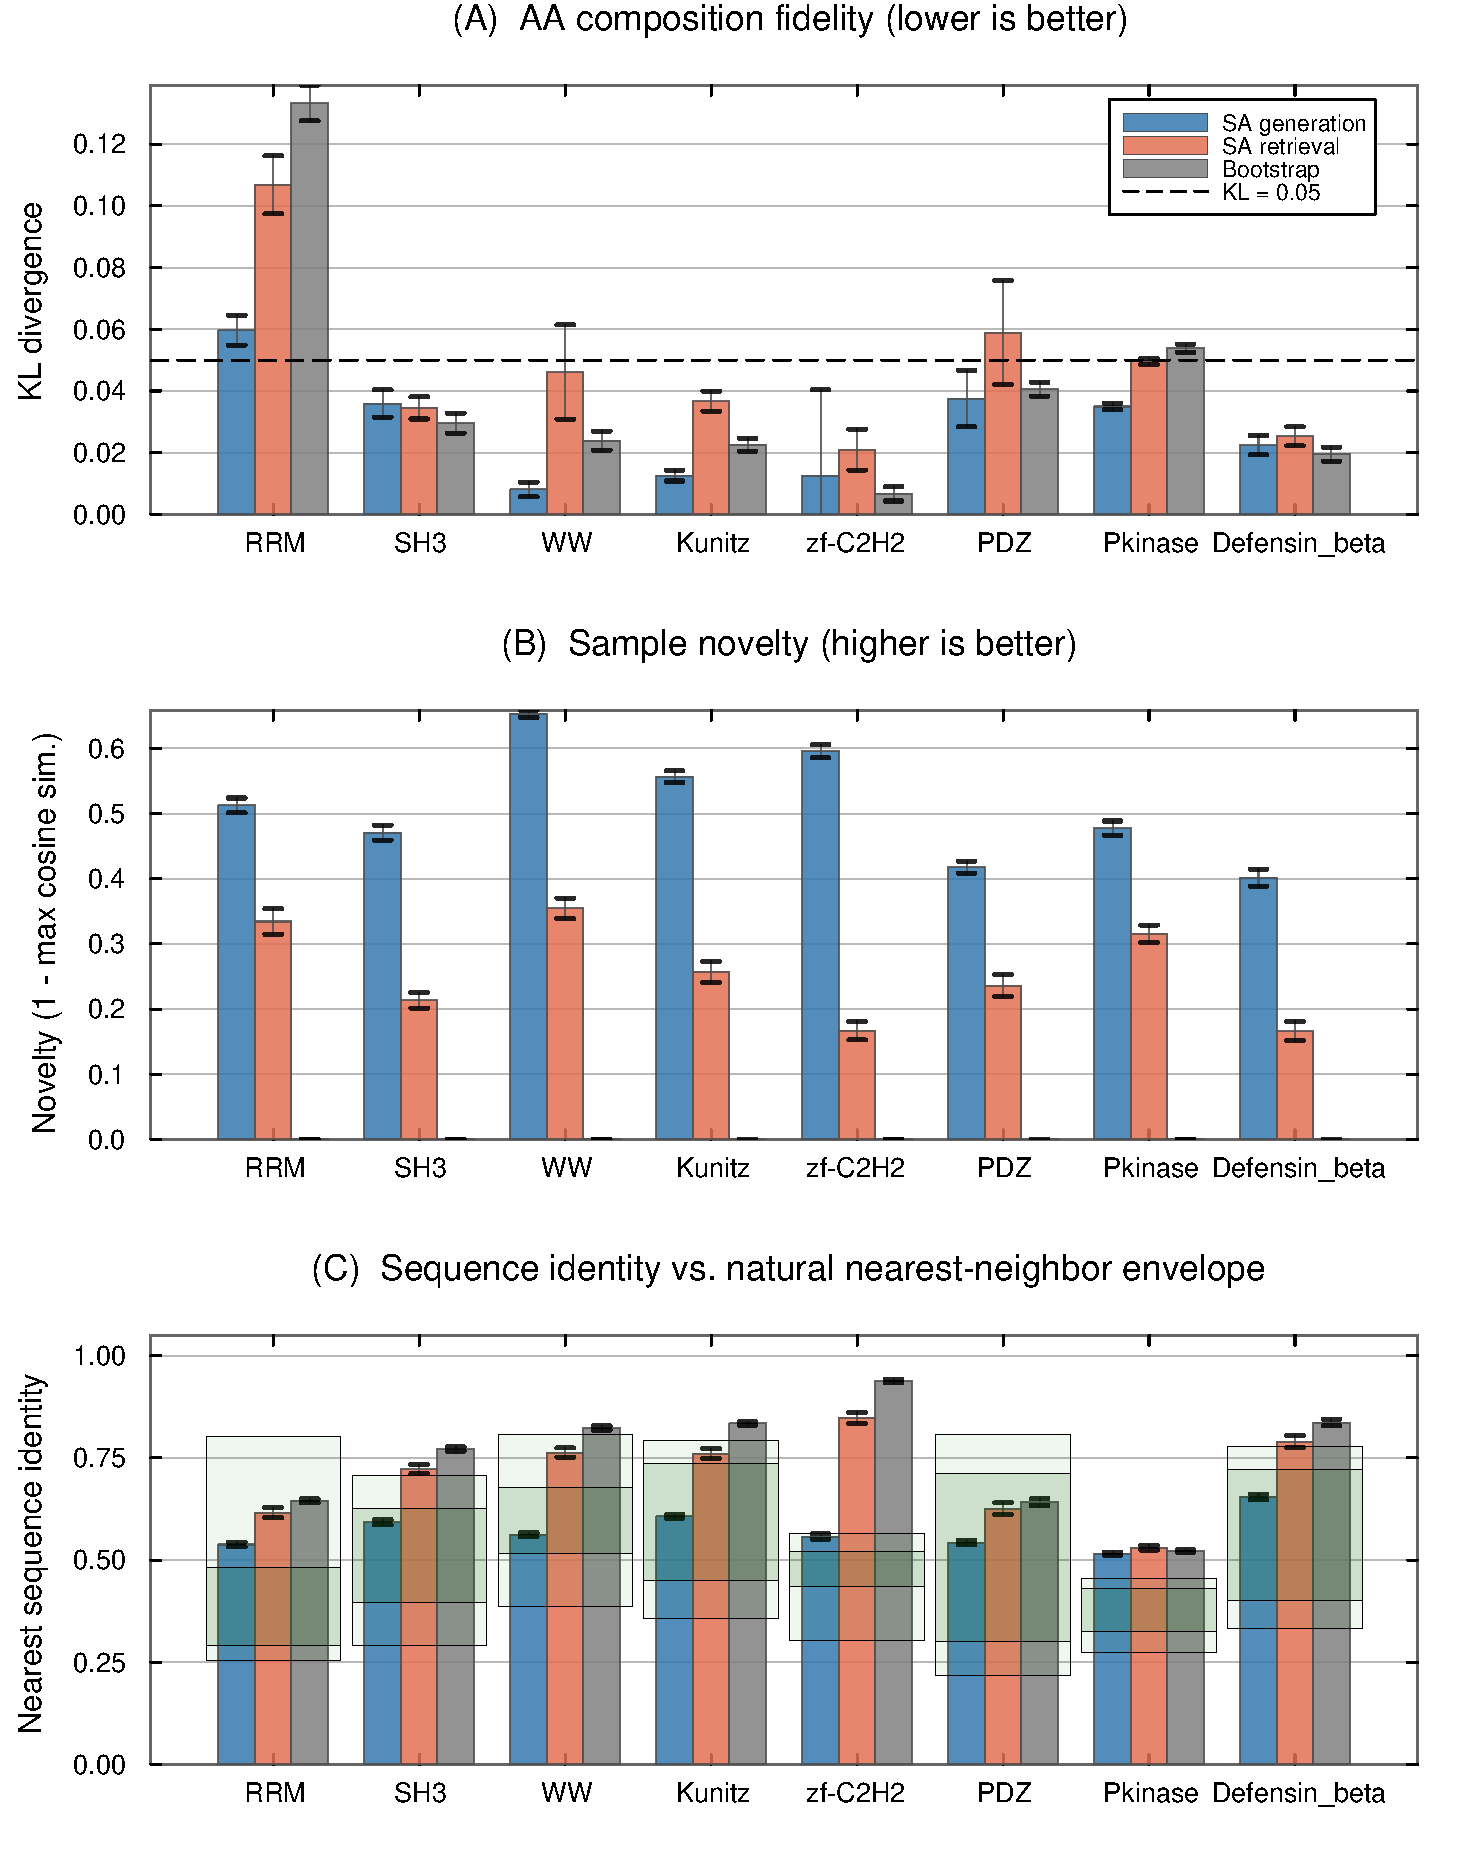
\includegraphics[width=0.9\textwidth]{figs/cross_family_composite.pdf}
\caption{Cross-family comparison of SA generation, SA retrieval, and bootstrap across eight Pfam families. \textbf{(A)}~KL divergence of amino acid composition (lower is better); dashed line at KL${=}0.05$ marks the practical threshold below which deviations are indistinguishable from finite-sample variation. SA generation achieves the lowest or near-lowest KL in every family. \textbf{(B)}~Novelty in PCA space ($1 - \max_k \cos(\hat{\xi}, \mathbf{m}_k)$; higher is better). SA generation produces substantially novel sequences, while bootstrap samples, which are exact copies of stored patterns, have zero PCA-space novelty by construction. \textbf{(C)}~Nearest sequence identity to a stored pattern; the green shaded band (30--70\%) marks the typical within-family identity range; sequences below this band have drifted outside the family, while sequences above it are near-copies of stored patterns with insufficient novelty. SA generation falls within this range across all eight families. Error bars show $\pm 1$ SE (30 chains $\times$ 5 samples).}
\label{fig:cross-family}
\end{figure}

\begin{figure}[p]
\centering
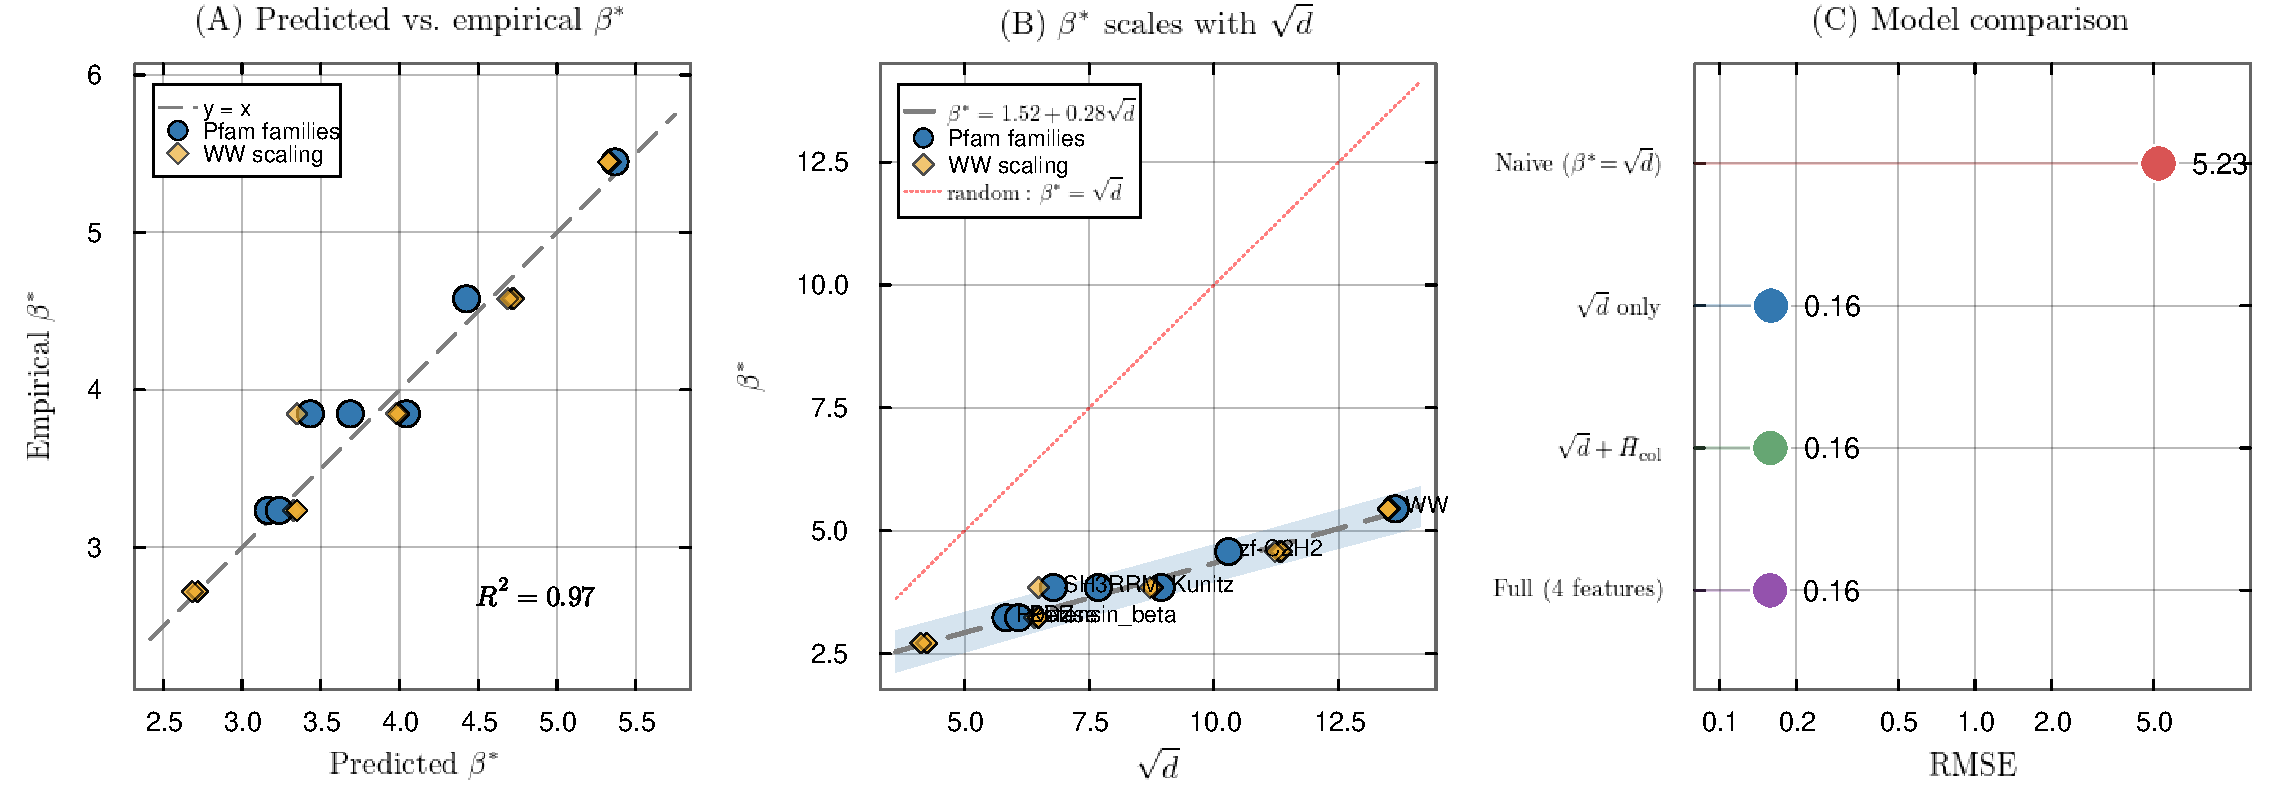
\includegraphics[width=\textwidth]{figs/beta_prediction_composite.pdf}
\caption{Predicting the critical temperature from MSA statistics. \textbf{(A)}~Predicted vs.\ empirical $\beta^*$ for the simple linear model $\beta^* \approx 1.57 + 0.28\sqrt{d}$ ($R^2{=}0.97$, $n{=}33$). Blue circles: eight Pfam families; gold diamonds: WW scaling replicates ($K \in \{20,\ldots,400\}$, five repeats each). \textbf{(B)}~$\beta^*$ as a function of $\sqrt{d}$, with the fitted regression (dashed) and the random-pattern prediction $\beta^* = \sqrt{d}$ (dotted red). The intercept offset and reduced slope reflect structured correlations in real protein families. \textbf{(C)}~Model comparison (log-scale RMSE). The fitted two-parameter model (RMSE${=}0.16$) is $33\times$ more accurate than the naive random-pattern prediction $\beta^* = \sqrt{d}$ (RMSE${=}5.29$); adding MSA features provides negligible improvement.}
\label{fig:beta-prediction}
\end{figure}

\begin{figure}[p]
\centering
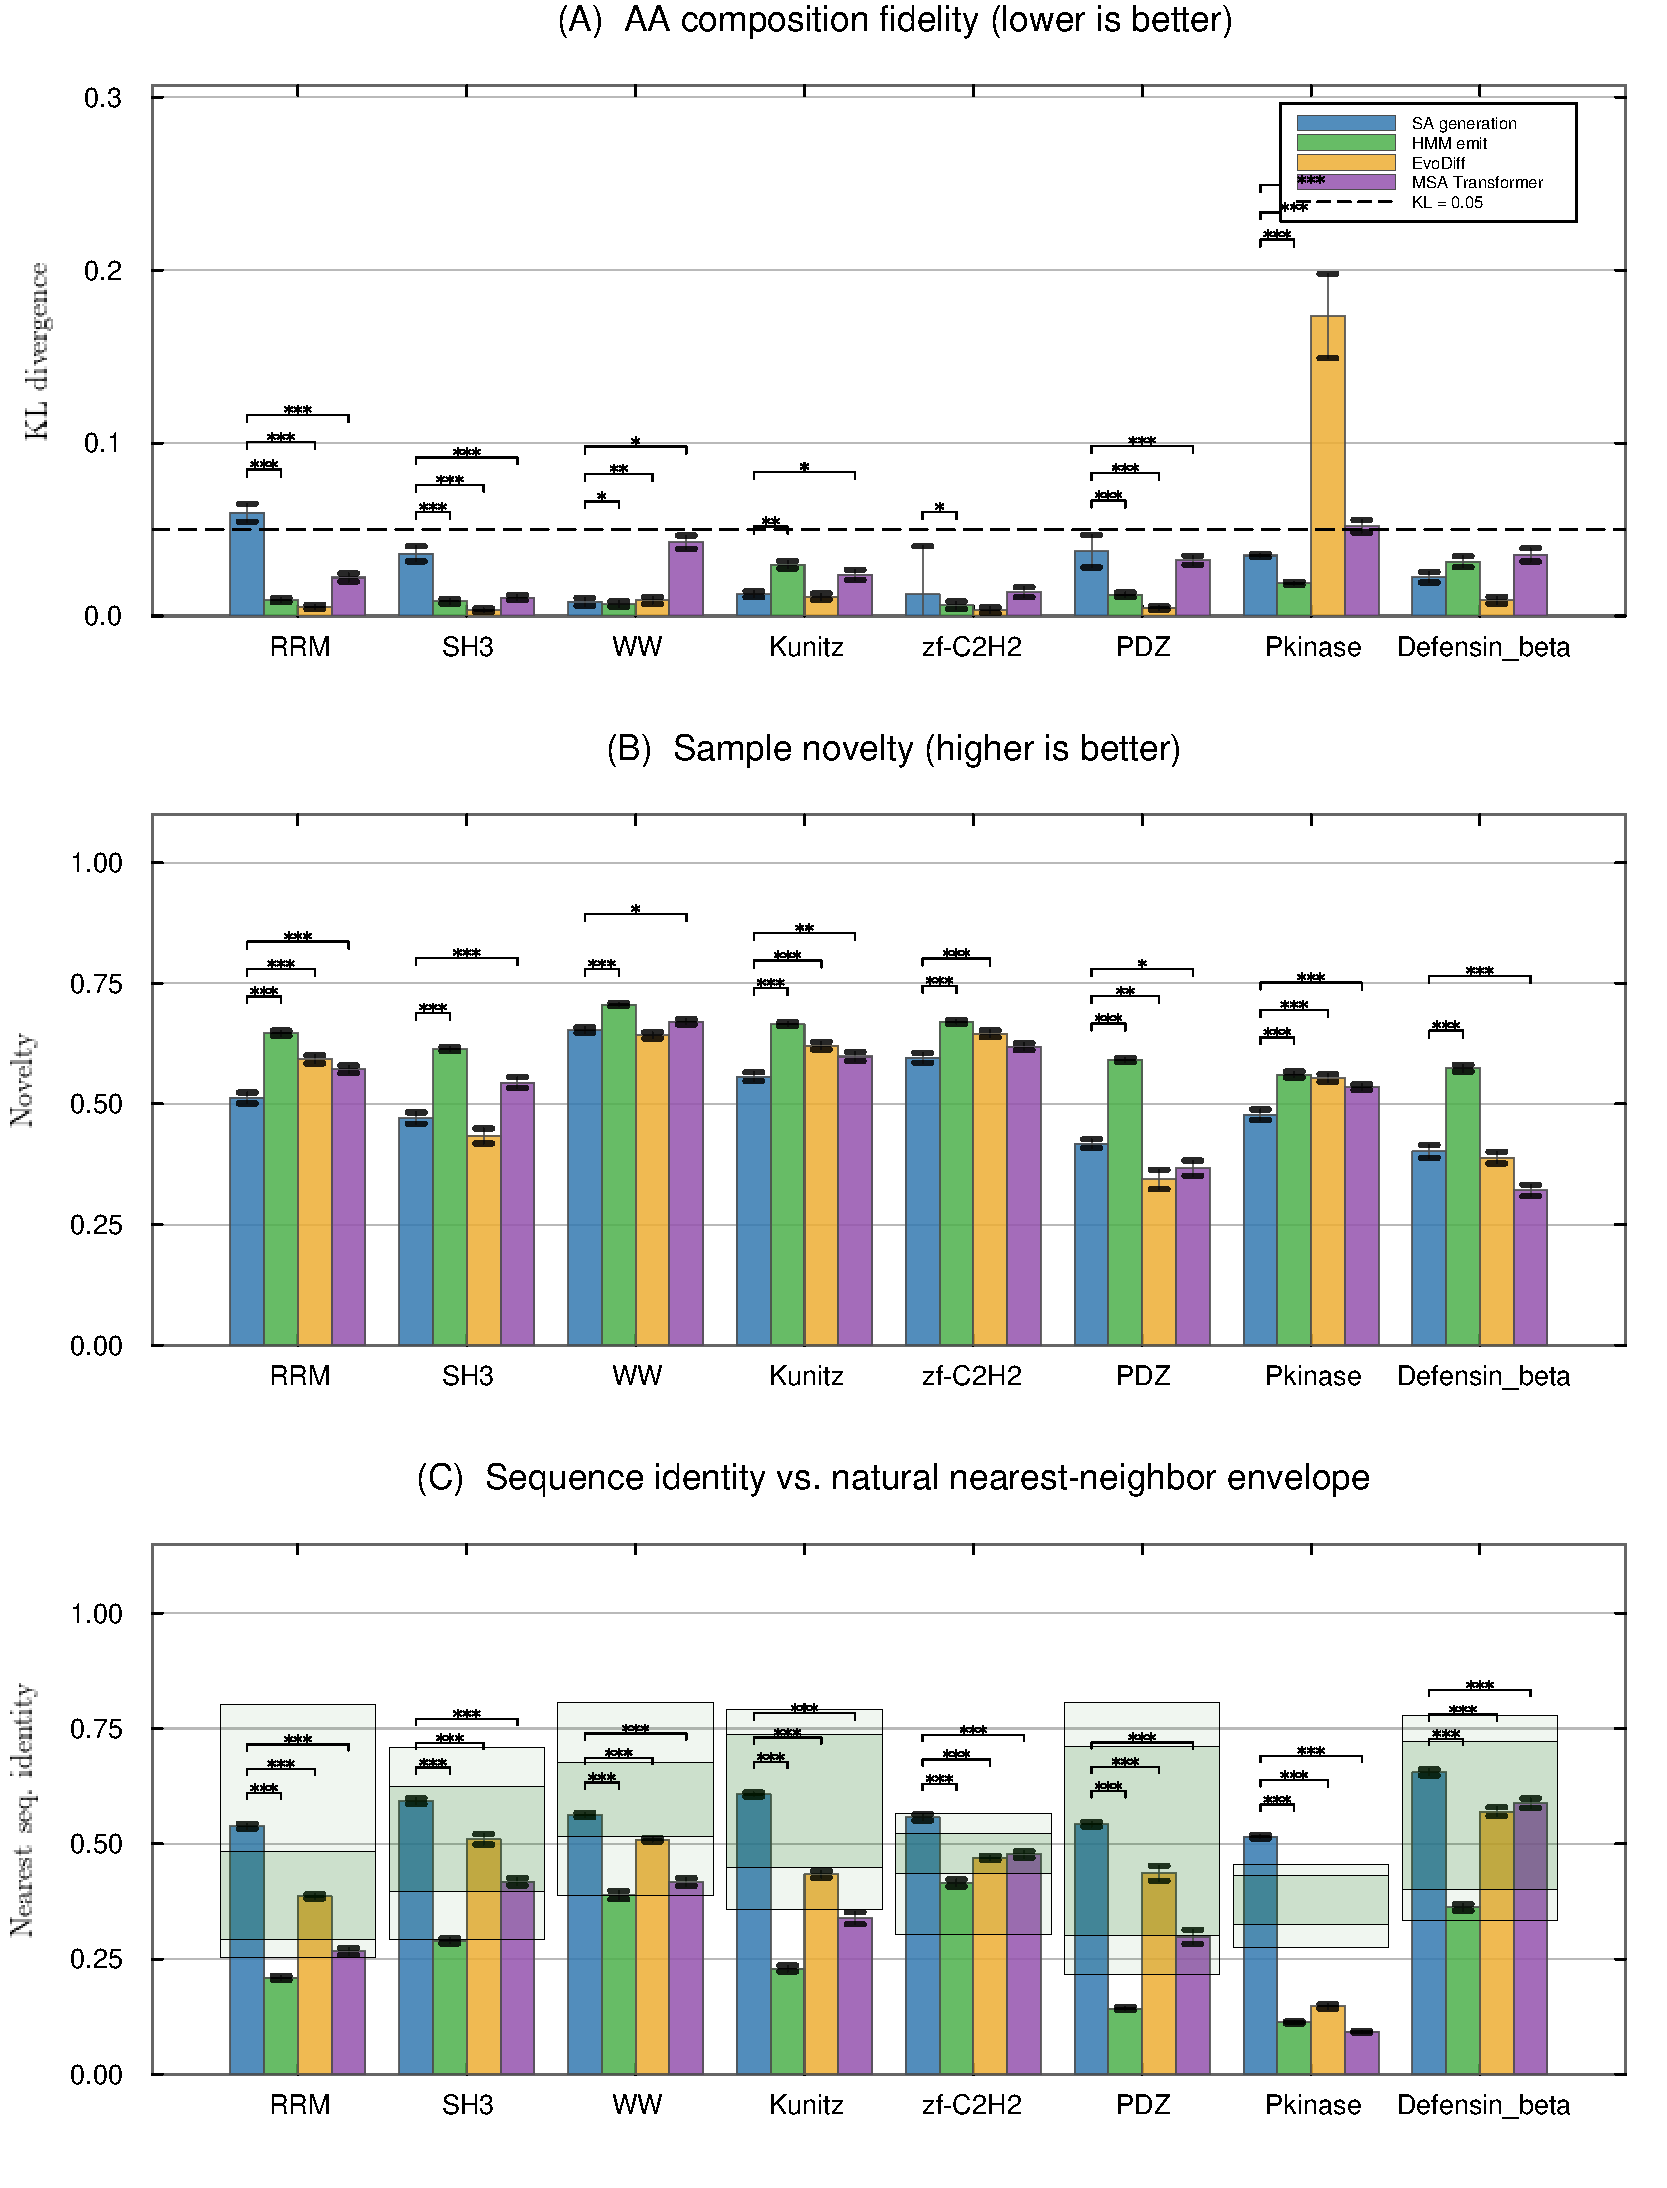
\includegraphics[width=0.85\textwidth]{figs/baseline_comparison_composite.pdf}
\caption{Head-to-head comparison of SA generation against three learned baselines (profile HMM emit, EvoDiff, MSA Transformer) across all eight Pfam families. \textbf{(A)}~KL divergence of amino acid composition (pooled over all 150 generated sequences, with bootstrap SE; $n_{\mathrm{boot}}{=}1000$); dashed line at KL${=}0.05$ marks the threshold below which deviations are indistinguishable from finite-sample variation. \textbf{(B)}~Novelty in PCA space. \textbf{(C)}~Nearest sequence identity to a stored pattern; the green shaded band (30--70\%) marks the typical within-family identity range; sequences below this band have drifted outside the family, while sequences above it are near-copies of stored patterns with insufficient novelty. Panels (B) and (C) report per-chain means $\pm 1$ SE (30 chains $\times$ 5 samples). Significance brackets show Wilcoxon rank-sum tests comparing SA generation to each baseline (HMM emit, EvoDiff, MSA Transformer); only significant comparisons are shown ($^{***}p < 0.001$, $^{**}p < 0.01$, $^{*}p < 0.05$). Simple reference baselines (Gaussian perturbation, convex combination, stored-pattern retrieval) are omitted from this figure because their design precludes meaningful comparison; their metrics are reported in SI Appendix, Table~S1 for completeness.}
\label{fig:baseline-comparison}
\end{figure}

\begin{figure}[p]
\centering
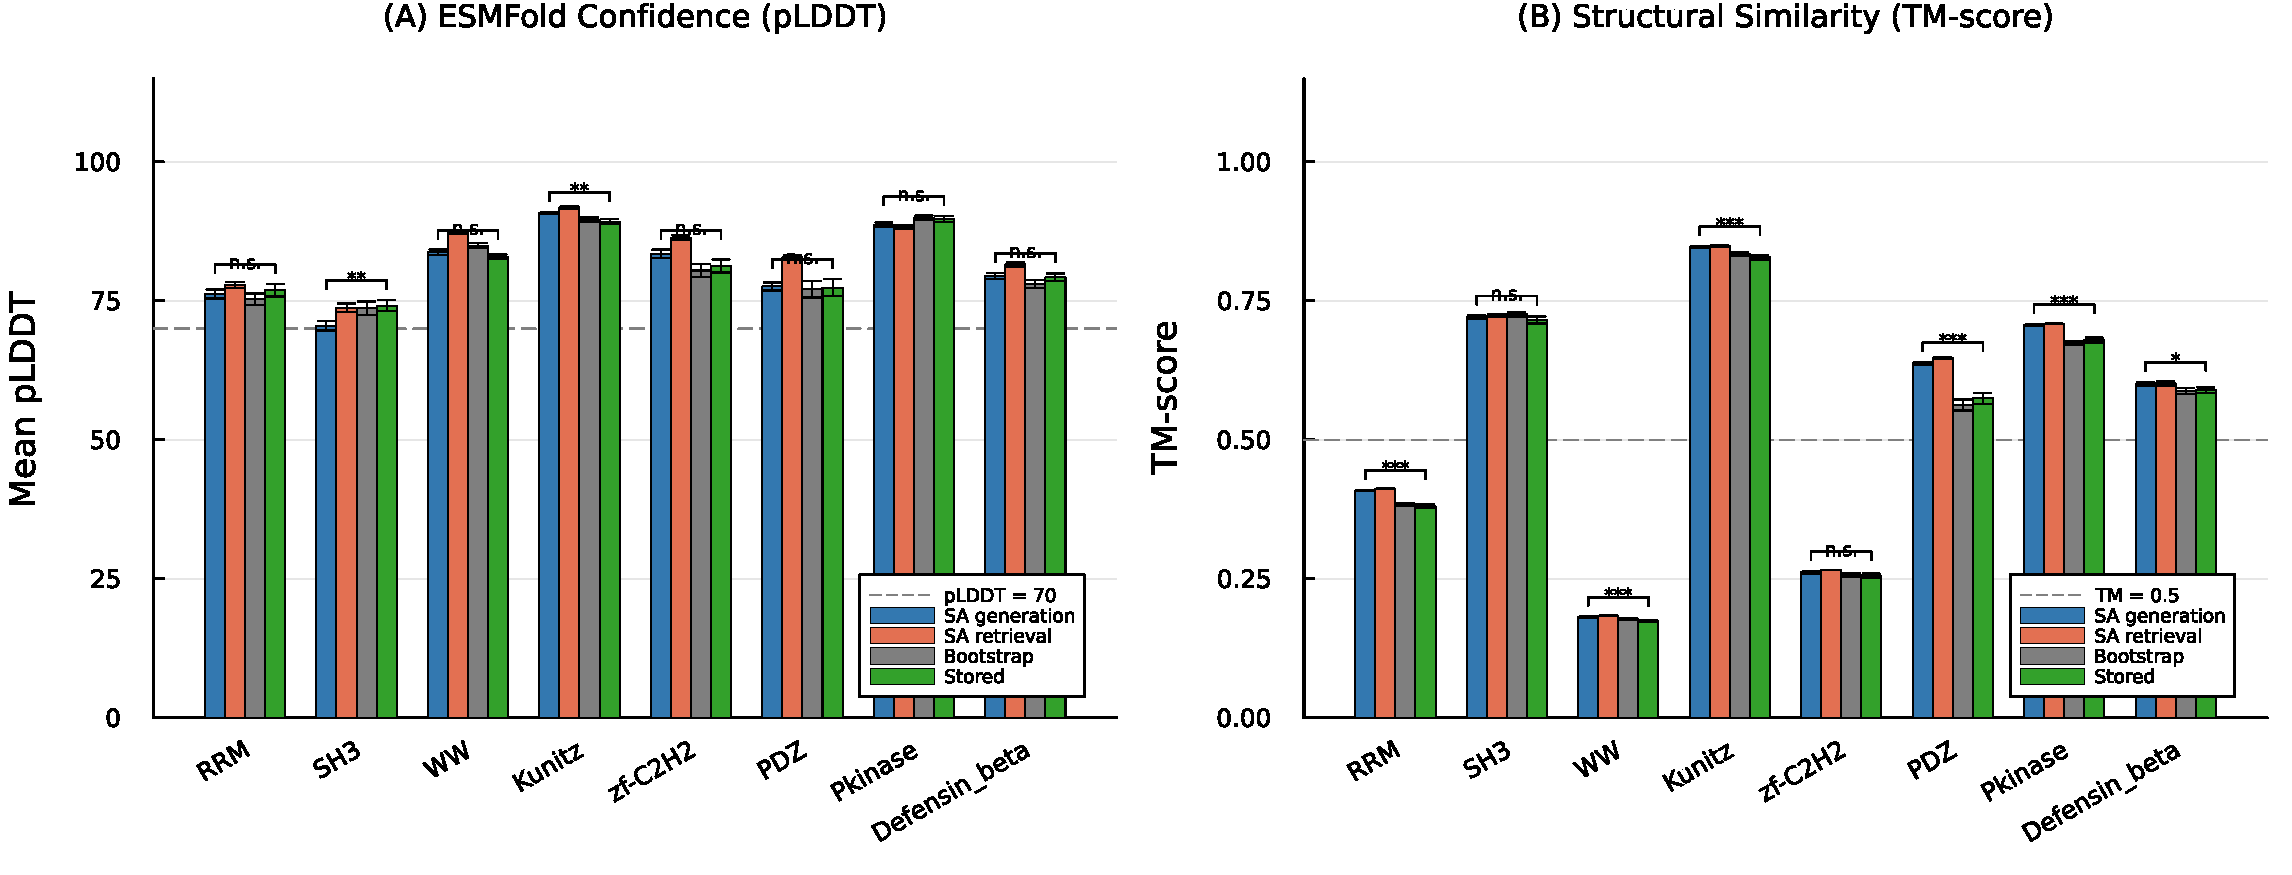
\includegraphics[width=0.9\textwidth]{figs/structure_validation_composite.pdf}
\caption{Structure validation of SA-generated sequences using ESMFold. \textbf{(A)}~Mean pLDDT (folding confidence) across all eight Pfam families for SA generation, SA retrieval, bootstrap, and stored (natural) sequences. The dashed line indicates the pLDDT${=}70$ confidence threshold. \textbf{(B)}~TM-score to a representative experimentally determined structure for each family. The dashed line indicates TM${=}0.5$ (same-fold threshold). Significance brackets show Wilcoxon rank-sum tests comparing SA generation to stored sequences: $^{***}p < 0.001$, $^{**}p < 0.01$, $^{*}p < 0.05$, n.s.\ = not significant. Error bars show $\pm 1$ SE ($n{=}50$ sequences per condition).}
\label{fig:structure-validation}
\end{figure}

\begin{figure}[p]
\centering
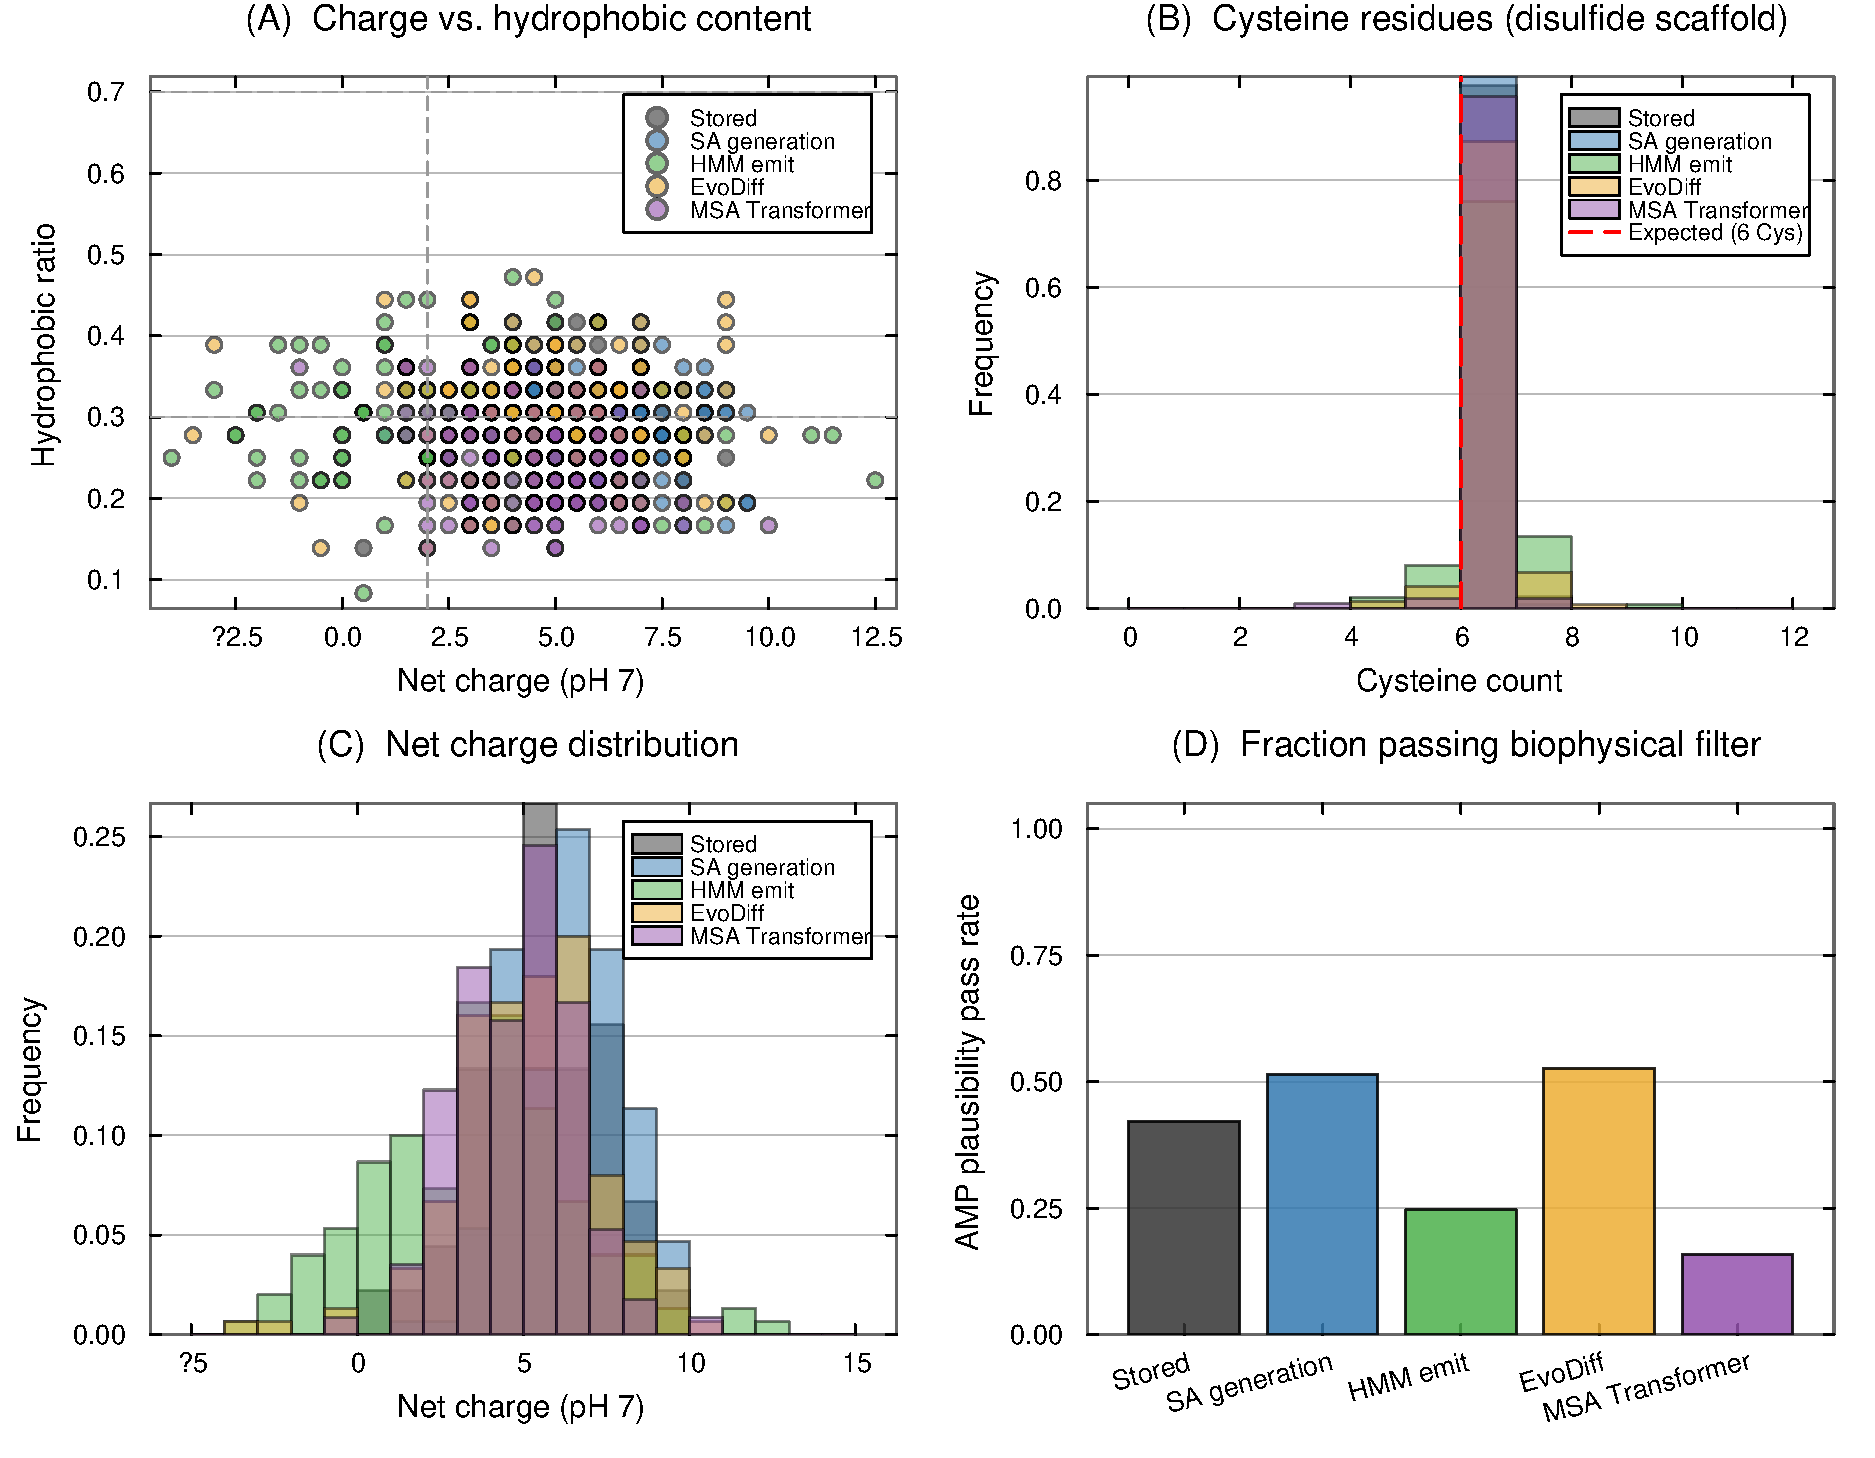
\includegraphics[width=0.9\textwidth]{figs/defensin_biophysics.pdf}
\caption{Biophysical properties of beta defensin sequences (PF00711). \textbf{(A)}~Net charge at pH~7 vs.\ hydrophobic residue fraction. SA-generated sequences (blue) overlap the stored natural sequences (gray), while HMM emit (green) and MSA Transformer (purple) drift to lower charge. Dashed lines indicate the antimicrobial plausibility thresholds (charge $\geq +2$, hydrophobic fraction $0.3$--$0.7$). \textbf{(B)}~Cysteine count distribution. SA generation preserves the six-cysteine disulfide scaffold (red dashed line) with the same fidelity as the stored alignment. \textbf{(C)}~Net charge distribution. SA generation produces a charge profile closely matching stored sequences. \textbf{(D)}~Fraction of sequences passing a minimal biophysical plausibility filter (charge $\geq +2$, hydrophobic fraction $\in [0.3, 0.7]$, $\geq 4$ cysteines).}
\label{fig:defensin-biophysics}
\end{figure}

\begin{figure}[p]
\centering

\includegraphics[width=0.9\textwidth]{figs/structure_gallery.pdf}
\caption{AlphaFold2 predicted structures for representative SA-generated sequences (colored by per-residue pLDDT confidence) superimposed on the experimentally determined reference structure for each family (gray, semi-transparent). For each family, the SA-generated sequence with the highest mean pLDDT was selected and aligned to the reference using PyMOL. The close predicted structural agreement (sub-angstrom root-mean-square deviation (RMSD)) and uniformly high pLDDT scores are consistent with SA-generated sequences encoding three-dimensional folds that recapitulate the canonical architecture of their target family, despite $40$--$65\%$ sequence novelty.}
\label{fig:structure-gallery}
\end{figure}

\end{document}
